\documentclass[a4paper,oneside]{memoir}


\usepackage[utf8]{inputenc}
\usepackage[T1]{fontenc}

\usepackage{lmodern}



%\usepackage[czech]{babel}
\usepackage{amsmath,amssymb,mathtools,amsthm,bm}

\usepackage{xspace}


\usepackage{lipsum}

\usepackage{hyperref}
\hypersetup{
    colorlinks,
    citecolor=black,
    filecolor=black,
    linkcolor=black,
    urlcolor=black
}

%\usepackage{enumitem}

\title{TFGP readme}

\author{Tomáš Křen}

\hyphenation{vě-dec-ká}

\begin{document}

\theoremstyle{plain} 
\newtheorem{theorem}{Theorem} 
\newtheorem{proposition}{Proposition} 
\newtheorem{lemma}{Lemma} 
\newtheorem{preLemma}{Pre-Lemma} 
\newtheorem*{corollary}{Corollary}

\theoremstyle{definition} 
\newtheorem*{definition}{Definition} 
\newtheorem*{preDefinition}{Pre-Definition} 
\newtheorem{conjecture}{Conjecture}
\newtheorem*{example}{Example} 

\theoremstyle{remark} 
\newtheorem*{remark}{Remark} 
\newtheorem*{note}{Note} 
\newtheorem{case}{Case}

\frontmatter
\mainmatter
\maketitle

%\renewcommand{\chaptername}{Akt}

\tableofcontents*
%\clearpage

\newcommand{\red}[1]{{\color{red} #1}}



\newcommand{\sigmaPr}{\sigma^\prime}
\newcommand{\tauPr}{\tau^\prime}
\newcommand{\xPr}{x^\prime}
\newcommand{\nPr}{n^\prime}
\newcommand{\nPrr}{n^{\prime\prime}}
\newcommand{\nPrrr}{n^{\prime\prime\prime}}
\newcommand{\tausPr}{\tau_s^\prime}
\newcommand{\s}{\sigma}
\newcommand{\Th}{\theta}
\newcommand{\sPr}{\sigmaPr}
\newcommand{\thPr}{\theta^\prime}



\newcommand{\then}{\Rightarrow}
\newcommand{\E}[2]{(\exists #1)\ #2}
\newcommand{\A}[2]{(\forall #1)\ #2}
\newcommand{\Ain}[3]{(\forall #1 \in #2)\ #3}


\newcommand{\op}{\operatorname}

\newcommand{\ar}{\rightarrow}
\newcommand{\ap}[2]{(#1\,#2)}
\newcommand{\defi}{\coloneqq}
\newcommand{\defe}{\mathrel{\vcentcolon\equiv}}

\newcommand{\binRule}[3]{\dfrac{#1\ ,\ #2}{#3}}
\newcommand{\triRule}[4]{\dfrac{#1\ ,\ #2\ , \ #3}{#4}}
\newcommand{\isSub}[1]{#1\ \mathit{substitution}}
\newcommand{\MGU}[2]{\op{MGU}(#1,#2)}
\newcommand{\mgu}[1]{\op{MGU}(#1)}

\newcommand{\AX}{\textit{AX}\xspace}
\newcommand{\subAx}{\textit{SUB-AX}\xspace}
\newcommand{\mguMp}{\textit{MGU-MP}\xspace}
\newcommand{\abs}[1]{\lvert #1 \rvert}




\chapter{i já it}

\section{Osnova}

\subsection{Mantry}

\textbf{Jak to napsat?}

- Jako bych psal TFGP blogísek, todle je trénink.

- Tak aby se to z toho pěkně pochopilo, ne aby to bylo HC formální nečitelná píčovina.

~\\

\subsection{High-level osnova}

\textbf{Problém popisu dagů} : 

- workflows jsou dagy

- dagy jde popsat operacema skladající jiný dagy

\textbf{Parametricky polymorfní Typovej systém} : 

- chceme konstruovat jen korektní dagy

- chceme aby na sebe navazovali správně počty atd

\textbf{Aplikativní notace}

- klasicka představa je že funkce jsou ve vnitřních uzlech a jejich parametry jsou syni

- aplikativní notace využívá toho, že každou funkci si díky curringu mužu chápat jako fci 1 proměný. 

- pak mužu vzit stromovou reprezentaci explicitně zachycující jednotlivé aplikace

\textbf{Generování}

Dosud jsme popsali co je cílem tvořit, ted popíšem jak na to jdeme.

- 1. základ našeho přístupu: generuje strom pro danou velikost stromu (počet symbolů).
  
  - což mimojiné umožnuje mnohem přímější kontrolu nad tím, z jakého rozložení taháme naše jhedince 
  - zde popsat to jak to děláme (32, 16,16, 8,8,8,8, ...)

- 2. základ našeho přístupu: počítáme si počty stromů pro jednotlivý dotazy 
     - abychom byli schopný generovat (semi-)uniformě

- 3. základ našeho přístupu: ex. sigma že z gamma de vyvodit že M je typu sigma(tau)

  - k tomu je potřeba definovat prerekvizitní pojmy, minimálně tyto:
    - substituce
    - a to jakym způsobem vypadá dotaz (k,tau) - a že je teda obecnejší to tau než přímo typ že pak M:Tau
      - to by šlo snad názorně ukázat na příkladě generování stromu k>1:
      - Generujem Dag D LD, k>1 -> v kořeni stromu je aplikace tedy:
         - levej syn je funkce z něčeho do (Dag D LD), pravej syn je to něco

  - to kulminuje v hodící se funkci subs, která pro danej dotaz (k,tau) vrátí substituce spolu s počtama stromů


- \textit{vygenerování jednoho jedince/stromu/programu}

 - (a) strom velikosti 1 - výběr symbolu z gammy aby to pasovalo
 - (b) strom velikosti k>1 - tedy jde o aplikaci a

- \textit{předpočítání pomocných dat pro generování}


- "semi-unfiromní" generování - poznámka o nedokonalosti v uniformitě

~\\

~\\

\subsection{Low-level osnova}

- Čim začít: 
Co je to ml workflow. 
ML workflows přirozeně tvoří graf. 
Natrénovat a vyhodnotit takový ensamble je to výpočetně náročný a tak chceme vyloučit cykly. 
Tedy budeme tvořit dagy. 

Architektura našeho systému sestává ze dvou základních úkolů:
(1) Vytvořit DAG reprezentující daný workflow - pomocí evoluce by GP
(2) Natrénovat a vyhodnotit daný workflow

Během evoluce však nepracujemes přímo s grafovou reprezentací ale nepřímo skrze stromovou reprezentaci programu, jehož výsledkem je DAG popisující daný workflow.

Tedy jsou to 3 kroky: strom popisuje program který když se vyhodnotí tak jeho výsledek je graf podle kterého se postavý ML workflow který se natrénuje a vyhodnotí.


Základní stavební bloky jsou basic klasifikační metody.
Dálešími elementárními prvky jsou jedotlivé preprocessingy, clusteringy a votovací metody. 
Každou z elementárních metod můžeme chápat jako dag.
Tyto elementární prvky jsou kombinovány do větších pomocí operací skladajících dva a víc menších dagů do jednoho většího.

 


Výsledkem prvního kroku je tedy graf. 
To jak zacházíme s Při vytváření daného , ten však může být výsledkem  

My ale
Dagy reprezentujeme jako výrazy.

- Co je jádro:

- Jak to schrnout:

~\\



\section{Our approach}


\newcommand{\Dlong}{unlabeled data\xspace}
\newcommand{\LDlong}{labeled data\xspace}
\newcommand{\Dshort}{\textit{$D$}\xspace}
\newcommand{\LDshort}{\textit{$LD$}\xspace}
\newcommand{\dia}{\textit{$ens_1$}\xspace}
\newcommand{\diaZero}{\textit{$ens_0$}\xspace}
\newcommand{\splitComb}{\textit{$split$}\xspace}
\newcommand{\cons}{\textit{$cons$}\xspace}

\newcommand{\komb}[1]{\textit{#1}}
\newcommand{\kons}[1]{\textbf{#1}}

\newcommand{\Dag}{\kons{Dag}}
\newcommand{\D}{\kons{D}}
\newcommand{\LD}{\kons{LD}}
\newcommand{\Boo}{\kons{Boo}}
\newcommand{\V}{\kons{V}}
\newcommand{\Succ}{\kons{S}}
\newcommand{\Zero}{\kons{0}}
\newcommand{\Same}{\kons{Same}}
\newcommand{\Disjoint}{\kons{Disjoint}}

\newcommand{\Suc}[1]{(\Succ\ #1)}
\newcommand{\Ve}[3]{(\V\ #1\ #2\ #3)}

\newcommand{\DAG}[2]{(\Dag\ #1\ #2)}
\newcommand{\splitter}[4]{\DAG{#1}{\Ve{#2}{#3}{#4}}}
\newcommand{\merger}[4]{\DAG{\Ve{#1}{#3}{#4}}{#2}}
\newcommand{\dvaPlus}[1]{\Suc{\Suc{#1}}}
\newcommand{\dva}{\dvaPlus{\Zero}}


\red{Nasleduje rozdelana verze our approache, jeste to budu dost menit, tak se nelekejte, nebude tam tolik nadpisu nebude tam nic cesky atd.}

\subsection{Individual representation}

\subsubsection{What is a machine learning workflow?}
Let us start with brief clarification of what we mean by term machine learning workflow. We can distinguish two kinds of machine learning methods: basic and combined. The basic methods are particular \textit{named} methods such as specific classification, regression, clustering, preprocessing or voting algorithms. On the other hand, the combined methods are \textit{anonymous} results of combining several basic methods into one compound by means of some specific ensemble method (such as stacking or boosting) or by simply putting outputs of one method as inputs to other ones. We call these combined method \textit{machine learning workflows}.

\subsubsection{ML workflows as graphs}
ML workflows are naturally representable as directed graphs; vertices represent basic methods and edges represent flows of data.
Figure xxx. shows an example of such a workflow containing all above mentioned kinds of basic methods and ensembles.

[Example picture with everything]

Each edge has a type corresponding to the type of data flowing through it. 
From the high level machine learning point of view we distinguish two basic types o data;
input \Dlong ($\D$) and output \LDlong ($\LD$) containing the predictions.

Workflow graphs are slightly different from standard graphs in that some of the edges may start nowhere (input edges) or end nowhere (output edges). 
Alternatively we may add two special nodes, \textit{input} and \textit{output}, and let these special edges star or end in them.
One way or another, the special edges determine a \textit{type} of a workflow.

A workflow (such as the one on fig. xxx.) representing a classifier has one input edge of type $\D$ and one output edge of type $\LD$.

To train and evaluate a significant number of such workflows - which may possibly be rather huge beasts -  presents a seriously time consuming task (thanks especially to nested cross-validations). Therefore we decided to take into account only workflows without cycles in their graph, i.e. directed acyclic graphs (DAGs). Doing so we limit the training and evaluation time by limiting the size of generated workflows, since the evaluation time of a DAG workflow is reasonably proportional to the number of basic methods.

Consider a DAG with one input edge of type $a$ and with one output edge of type $b$, then we say that the dag has type $\DAG{a}{b}$. 
For example the DAG from fig. xxx has type $\DAG{\D}{\LD}$ which is the type of a classifier.
Type $\Dag$ is an example of a \textit{parametric type}, that is a type that takes two other types (e.g. $\D$ and $\LD$) as parameters to construct a specific type (e.g. $\DAG{\D}{\LD}$).
Parametric types are extensively used and exploited in our approach.
To deal with DAGs with multiple input or output edges is a slightly more complicated business explained below.

\subsubsection{DAG combinators}

During the evolution we need to generate and manipulate the workflow individuals. Rather than direct manipulation of the DAGs we prefer an indirect tree representation. From the evolution point of view the individuals are program expressions that may be  evaluated to give a value. This value is a JSON\footnote{Javascript object notation \red{jednou vetou popsat mozna}.} representation of the DAG encoding a ML workflow. This JSON value serves as a blueprint from which the actual ML workflow is build. Thus the DAG representation is an intermediate representation of a workflow.

Our approach to constructing the workflow DAGs is based on strongly typed pure functional programming style. In the terms of classical genetic programming, one specifies a library from which the syntactic trees of program individuals are build by specifying a set of terminals (leaf node symbols) and a set of functions (interior node symbols). 

Roughly speaking, we may say that our terminal set consists of basic machine learning methods and function set consists of dag combinators; operators that connect two or more smaller DAGs in a single more complicated one by some kind of serial or parallel composition. A careful reader may spot that some higher-orderism is in order here, since basic methods are basically functions, thus DAG combinators are functions over functions, i.e. higher-order functions.

We see three major benefits of the tree representation of individuals in comparison with a more direct representation:

(1) Trees are simple yet rich enough structures to support natural ways of substructure manipulation satisfying recombination needs of evolution driven search. Most notably in a cross-over operator. 

(2) \red{Extensibility. Functional programming - simple yet powerful tool for writing extensible programs.}

(3) Satisfaction of semantically imposed constraints. Because not all the possible DAGs are meaningful ML workflows. We manage to satisfy these constraints by transforming them onto type level in a way which we are going to demonstrate on the following simple example.

\subsubsection{Generality and Correctness of the combinators}

In the case of classical untyped genetic programming the terminal and function set consists only of the symbols accompanied with information about number of arguments that each function takes. In the typed situation we accompany the symbols with their types. Since the information whether a symbol is a terminal or function (and its arity) is already contained in the types, we can marge the terminal and function set into one library\footnote{\red{poznamka o tom ze v typový teorii se tomu řika context or basis a tak to pouzivame aby se propojila souvyslost.}} set $\Gamma$. This merge is also natural for applicative tree notation we use, which is described below.  

Let us consider a small yet illustrative workflow depicted on figure \ref{simple_stacking} together with its tree representation, on which we demonstrate some of our combinators and why they have rather complicated types.

\begin{figure}[th]
\centerline{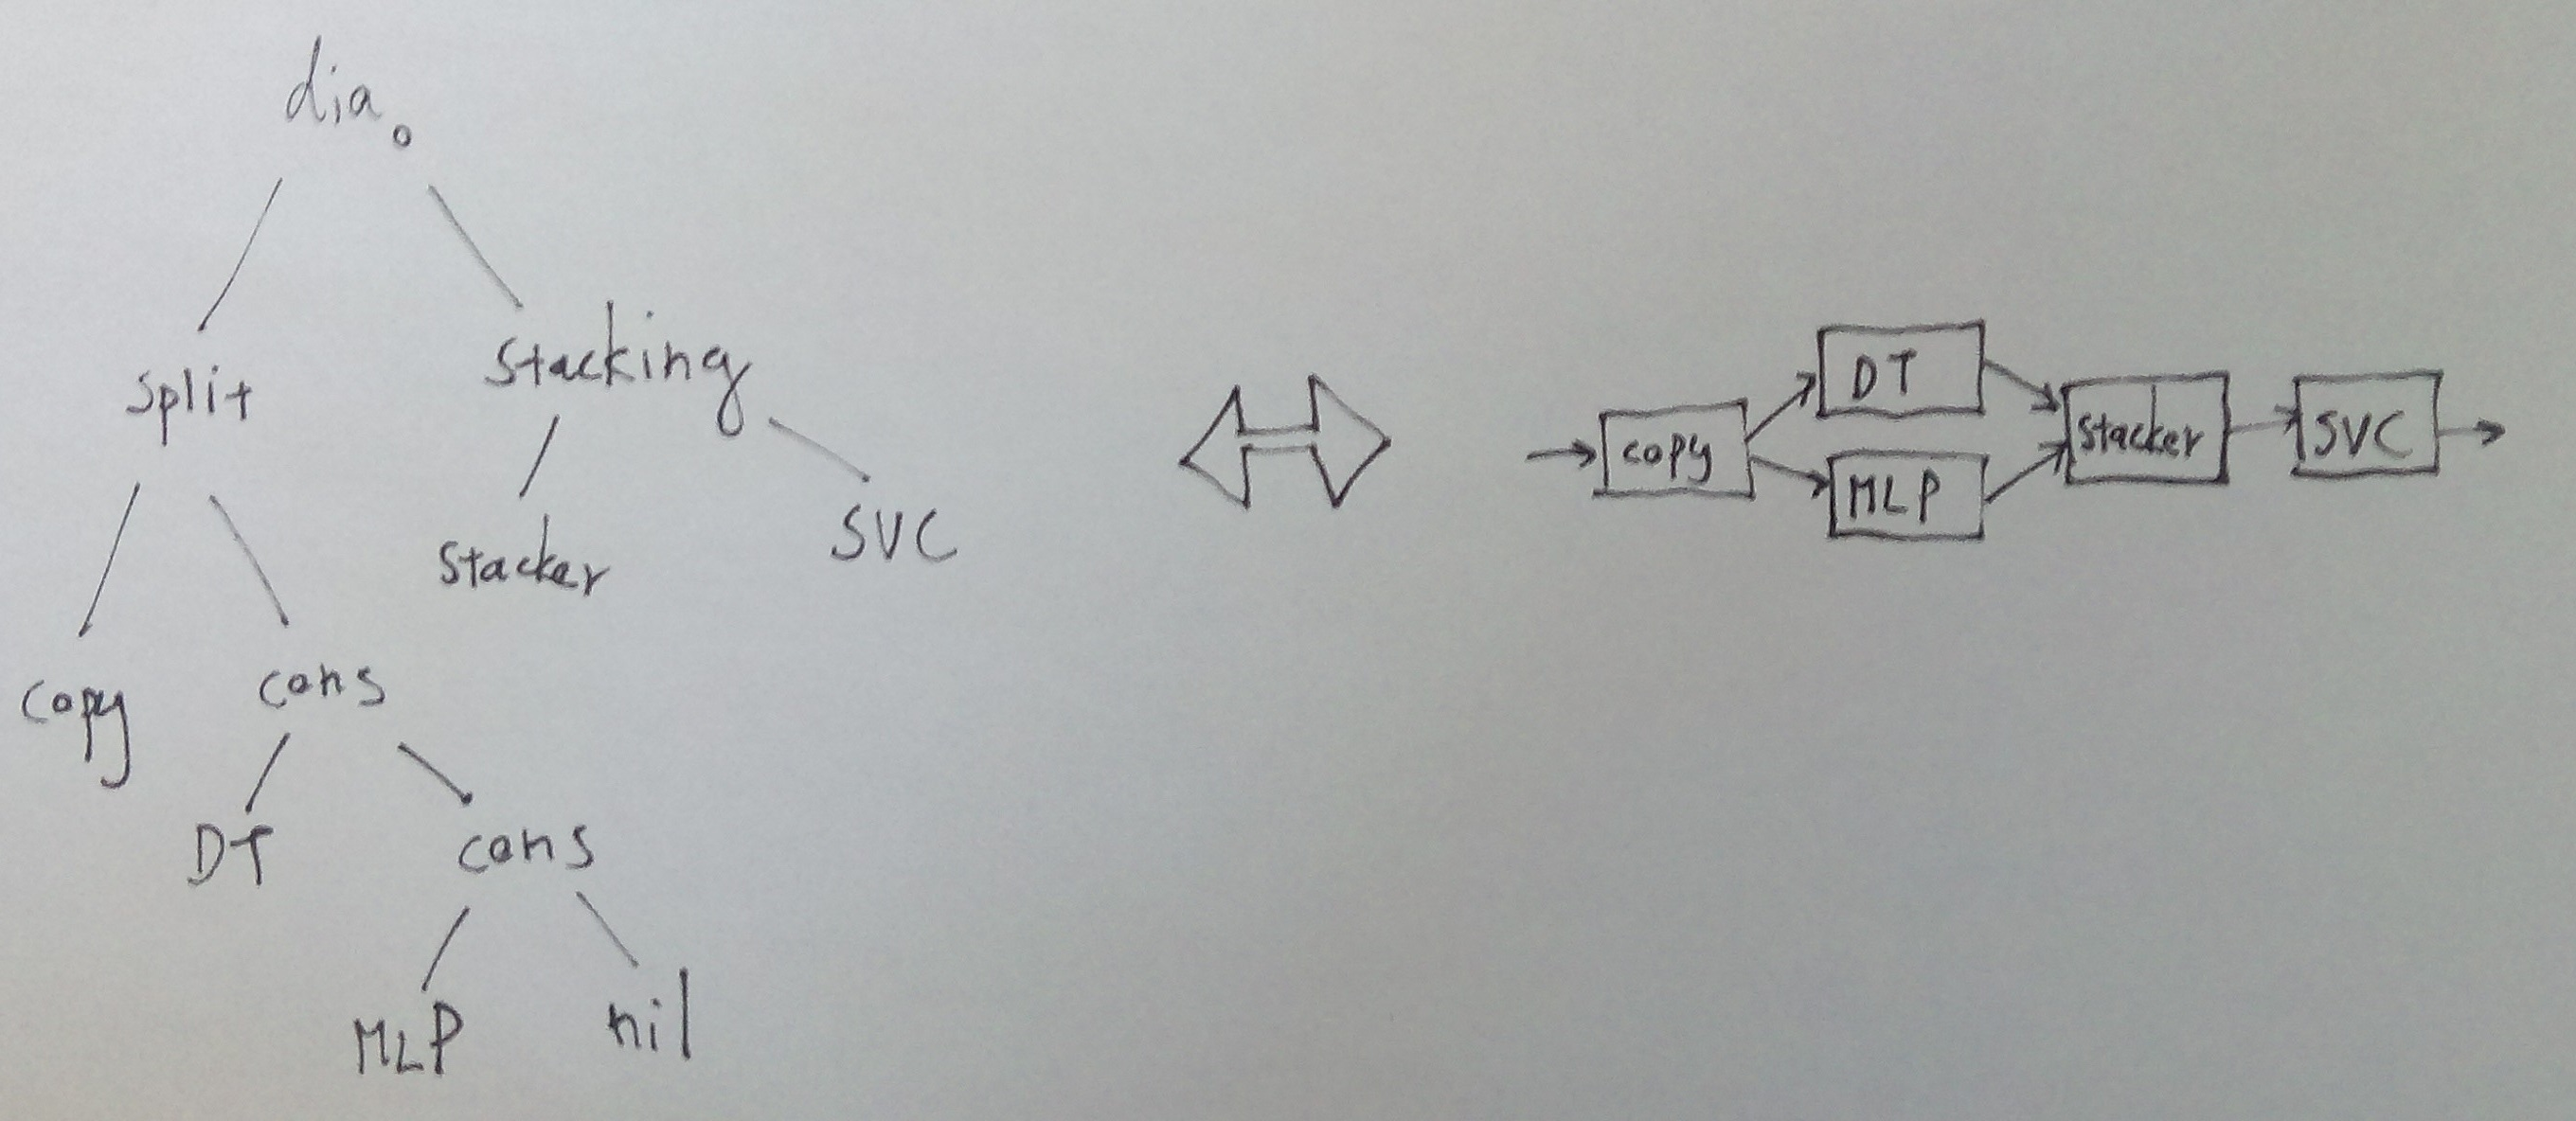
\includegraphics[width=10cm]{simple_stacking.jpg}}
\vspace*{8pt}
\caption{Simple stacking example.}
\label{simple_stacking}
\end{figure}

Although we internally use more general applicative tree representation (with all the symbols in leaf nodes),
here we present the tree as an S-expression with function symbols in the interior nodes.
Let us start in the root of the tree, where is the $dia_0$ symbol standing for DAG combinator with type:
 
$\splitter{\D}{\LD}{n}{c} \ar \merger{\LD}{\LD}{n}{c} \ar \DAG{\D}{\LD}$
  
So it is a function taking two arguments\footnote{we use the functional convention for functions with multiple arguments discussed below in the subsection about applicative notation}, 
first of type $\splitter{\D}{\LD}{n}{c}$ and second of type $\merger{\LD}{\LD}{n}{c}$, 
and producing result of type $\DAG{\D}{\LD}$, that is a DAG with one input edge of type $\D$ and one output edge of type $\LD$ representing a classifier model.
We use names starting with uppercase letter for specific (possibly parametric) types ($\Dag, \D, \LD, \V$) 
and names starting with lowercase letter for \textit{type variables} ($n, c$).

The result of the $dia_0$ combinator is a combined classifier workflow serially composing its two arguments, 
which are again workflows but now with a slightly more complicated type in the middle; 
the output type of the first and the input type of the second is the same type $\Ve{\LD}{n}{c}$. 




- ! predvest nad prikladem s jednoduchym stackingem, kde muzeme ukazat jak zakladni kombinátory, tak distinction of disjoint and copy data vector.
- Parametricky polymorfní Typovej systém
- chceme konstruovat jen korektní dagy
- chceme aby na sebe navazovali správně počty atd

We may say that our approach balances two mutually counteractive tendencies: generality and correctness.


\subsubsection{Applicative notation}

- klasicka představa je že funkce jsou ve vnitřních uzlech a jejich parametry jsou syni
- aplikativní notace využívá toho, že každou funkci si díky curringu mužu chápat jako fci 1 proměný. 
- pak mužu vzit stromovou reprezentaci explicitně zachycující jednotlivé aplikace

\subsection{Generating}

- Dosud jsme popsali co je cílem tvořit a co to omezuje, aby to dávalo smysl. Ted popíšem jak na to jdeme. Nejprve to ilustrujem jednoduchym prikladem to provide a context, pak formalneji predstavime general notions on which the approach is based and after that we describe the algorithm together with techniques which make it fast enough for massive use in generating and mutation.

\subsubsection{A simple example}

- to by šlo snad názorně ukázat na příkladě generování stromu k>1:
- Generujem Dag D LD, k>1 -> v kořeni stromu je aplikace tedy:
- levej syn je funkce z něčeho do (Dag D LD), pravej syn je to něco
… az se dostanem do listů (strom velikosti 1) - výběr symbolu z gammy aby to pasovalo..

\subsubsection{Existential queries}

- 1. základ našeho přístupu: ex. sigma že z gamma de vyvodit že M je typu sigma(tau)
  - k tomu je potřeba definovat prerekvizitní pojmy, minimálně tyto:
    - substituce
    - a to jakym způsobem vypadá dotaz (k,tau) - a že je teda obecnejší to tau než přímo typ že pak M:Tau

to kulminuje v hodící se funkci subs, která pro danej dotaz (k,tau) vrátí substituce spolu s počtama stromů


\subsubsection{Generating based on sizes}

- 2. základ našeho přístupu: generuje strom pro danou velikost stromu (počet symbolů).
  - což mimojiné umožnuje mnohem přímější kontrolu nad tím, z jakého rozložení taháme naše jhedince 
  - zde popsat to jak to děláme (32, 16,16, 8,8,8,8, ...)

\subsubsection{Counting the trees}

- 2. základ našeho přístupu: počítáme si počty stromů pro jednotlivý dotazy 
     - abychom byli schopný generovat (semi-)uniformě

\subsubsection{More involved example}

- jen pokud nebude stacit ten simple

\subsubsection{Final overview of generating}

- pridáme skolemizaci aby to fungovalo
- kesování aby se dalo generovat rychle
    - předpočítání pomocných dat pro generování
    - "semi-unfiromní" generování - pozn o nedokonalosti 
- kulminující v pseudokódu

\subsection{Formalization of our library}

- Ted když máme vybudovanou intuici pro to vo co tam de tak můžem na čtenář vyblít to co se na nějblije zhurta v ictai článku, s tim ze to muzem zestrucnit/zrychlit pac mnohe veci byly uz receny výše.




\chapter{Gecco}

\textbf{Uniform Generating for Strongly Typed Genetic Programming with Parametric Polymorphism}

In this paper we present a novel tree generating method for strongly typed genetic programming using a type system with parametric polymorphism. Our method is capable of uniform generating suitable both for a population initialization and a mutation operation. In order to perform this task effectively, the method utilizes type normalization and caching using dynamic programming. We concentrate on a deeper description of theoretical and technical aspects of our method to show its connection with logic programming. The method is demonstrated, analyzed and experimentally evaluated on a simple problem.


\chapter{Generating}

\section{General notions}

\begin{definition}
A $\mathit{term:type}$ statement $\mathit{M}:\mathit{\tau}$ states that (program) term $M$ has type $\tau$.   
A \textit{declaration} is a statement $s : \tau$ where $s$ is a term symbol and $\tau$ is a type.
Often we will write $s : \tau_s$ to emphasize that $\tau_s$ is the type of symbol $s$ in the supposed context.
A \textit{context} is set of declarations with distinct term symbols.\footnote{Interestingly, the definition of a \textit{context} and definition of a \textit{substitution} are almost the same. The difference is that "keys" in a context are term symbols/variables, whereas substitution "keys" are type variables. Maybe this fact could be utilized in an interesting way...}
\end{definition}


Suppose we have a context $\Gamma$. Let us consider $\mathit{term:type}$ statements derivable from the following rules (let us call them \subAx and \mguMp):

~

$\binRule{(s,\tau_s) \in \Gamma}{\isSub{\sigma}}{s : \sigma(\tau_s)}$
~~~
$\triRule{F : \tau_1 \ar \tau_2}{X : \tau^\prime_1}{\sigma \in \MGU{\tau_1}{\tau^\prime_1}}{\ap{F}{X} : \sigma(\tau_2)}$


\begin{definition}
Let $M$ be a term. Term size $\abs{M}$ is the number of symbols in $M$; e.g. $\abs{\ap{f}{\ap{\ap{g}{h}}{f}}} = 4$. 
\end{definition}

\newcommand{\inhab}[1]{\op{I}(#1)}

\newcommand{\tord}{\preccurlyeq}
\newcommand{\stord}{\prec}
\newcommand{\ordt}{\tord_\tau}
\newcommand{\tek}{\sim}
\newcommand{\ntek}{\nsim}
\newcommand{\ekt}{\tek_\tau}
\newcommand{\nekt}{\ntek_\tau}
\newcommand{\nsucct}{\nsucc_\tau}

\newcommand{\MGI}[1]{\op{MGI}(#1)}
\newcommand{\MGIt}{\MGI{\tau}}
\newcommand{\It}{\op{I}(\tau)}

\newcommand{\ids}{\sigma_{\op{id}}}

\newcommand{\U}[2]{\op{U}(#1,#2)}
\newcommand{\Utt}{\U{\tau}{\tauPr}}
\newcommand{\MGUtt}{\MGU{\tau}{\tauPr}}

\newcommand{\e}[2]{\op{E}_{#1}(#2)}
\newcommand{\restrict}[2]{{#1}_{\mid #2}}
\newcommand{\fresh}[2]{\op{fresh}_{#1}(#2)}
\newcommand{\newVar}[1]{\op{newVar}(#1)}
\newcommand{\Ss}[1]{\op{ss}(#1)}
\newcommand{\TS}[2]{\op{ts}_{#1}(#2)}
\newcommand{\ts}[2]{\op{ts}_{#1}(#2)}
\newcommand{\TSij}[3]{\op{ts}_{#1,#2}(#3)}
\newcommand{\trees}[2]{\op{trees}_{#1}(#2)}
\newcommand{\FX}{\ap{F}{X}}
\newcommand{\sF}{\s_{F}}
\newcommand{\sX}{\s_{X}}
\newcommand{\vars}[1]{\op{vars}(#1)}
\newcommand{\dom}[1]{\op{dom}(#1)}
\newcommand{\IH}{induction hypothesis\xspace}
\newcommand{\discup}{~\mathbin{\dot{\cup}}~}



\section{Reusable generating}

\begin{definition}
\begin{align*}
\e{k}{\tau} \defi& \{ M \mid \abs{M} = k, \E{\s}{ M : \s(\tau) } \} \\
\ts{1}{\tau,n} \defi&  \{ (s,\restrict{\mu}{\tau}, \nPr) \mid \\
 & ~~ (s,\tau_s) \in \Gamma, \\
 & ~~ (\tausPr,\nPr) = \fresh{\tau}{\tau_s, n}, \\
 & ~~ \mu = \mgu{\tau,\tausPr}
\} \\
\ts{i,j}{\tau,n} \defi& \{ (\FX, \restrict{(\sX \circ \sF)}{\tau}, \nPrrr) \mid \\ 
  & ~~ (\alpha, \nPr) = \newVar{\tau,n}, \\
  & ~~ (F,\sF,\nPrr) = \ts{i}{\alpha \ar \tau,\nPr}, \\
  & ~~ (X,\sX,\nPrrr) = \ts{j}{\sF(\alpha), \nPrr} 
\} \\
\ts{k > 1}{\tau,n} \defi& \bigcup\limits_{i=1}^{k-1}  \TSij{i}{k-i}{\tau, n}
\end{align*}
\end{definition}

\begin{lemma}[Core lemma about $\op{ts}_k$]
Let $(M, \s, \nPr) \in \ts{k}{\tau,n}$, then: 
\begin{align}
& \abs{M} = k,  
&\textit{(size)} \label{tsSize} \\
& M : \s(\tau), 
&\textit{(correctness)} \label{tsCorrectness} \\
& \A{\sPr}{M : \sPr(\tau) \then  \E{\theta}{\sPr(\tau) = \theta\circ\s(\tau)}},
& \textit{(generality)} \label{tsGenerality} \\
& \dom{\s} \subseteq \vars{\tau},\op{OK}(\tau,\nPr,\s), \nPr \geq n.
& \textit{(technical)} \label{tsTechnical}
\end{align}
\end{lemma}
\begin{proof}

By induction on $k$. 

Let $k = 1$. 
Let $(M, \s, \nPr) \in \ts{1}{\tau,n}$, 
then $M = s, \s = \restrict{\mu}{\tau}$,

where 
$(s,\tau_s) \in \Gamma,
(\tausPr,\nPr) = \fresh{\tau}{\tau_s, n},
\mu = \mgu{\tau,\tausPr}$.
 
(\ref{tsSize}) $\abs{M} = \abs{s} = 1$, since $s$ is a symbol of $\Gamma$.

(\ref{tsCorrectness}) From \textit{lemma about fresh$_\tau$} we have that 
$\E{\rho}{\rho(\tau_s) = \tausPr}$. 

Let us use (\AX) rule:
$\binRule{(s,\tau_s) \in \Gamma}{\isSub{\mu \circ \rho}}
{s : \mu(\rho(\tau_s))}$
\red{todo střízlivost}

Since $\mu = \mgu{\tau,\tausPr}$, we have $\mu(\tausPr) = \mu(\tau)$, 

therefore $\mu(\rho(\tau_s)) = \mu(\tausPr) = \mu(\tau) = \restrict{\mu}{\tau}(\tau)$, 

thus $s : \restrict{\mu}{\tau}(\tau)$.

(\ref{tsGenerality}) Let $\sPr$ be a substitution such that $s : \sPr(\tau)$.

From \textit{factoring lemma} we have that
$\E{\nu}{\nu(\tau) = \nu(\tausPr) = \sPr(\tau)}$. 

But $\mu = \mgu{\tau,\tausPr}$, thus 
$\mu$ is more general unification of $\tau$ and $\tausPr$ than $\nu$.

Therefore $\E{\theta}{\nu = \theta \circ \mu}$.

Finally $\sPr(\tau) = \nu(\tau) = \theta \circ \mu(\tau) = \theta \circ \restrict{\mu}{\tau} (\tau)$.

(\ref{tsTechnical}) Trivially $\dom{\restrict{\mu}{\tau}} \subseteq \vars{\tau}$.

\red{ todo zbytek technikálií (na papíře \#freshSummary)}.

Let $k > 1$. 

(\ref{tsSize})

(\ref{tsCorrectness})

(\ref{tsGenerality})

(\ref{tsTechnical})


\end{proof}


~\\

~\\

\section{Reusable generating - older approach}


\begin{definition}
\begin{align*}
\e{k}{\tau} &\defi \{ M \mid \abs{M} = k, \E{\s}{ M : \s(\tau) } \}   \\
\Ss{\tau}   &\defi \{ (s,\restrict{\mu}{\tau}) \mid (s,\tau_s) \in \Gamma, \mu = \MGU{\tau}{\fresh{\tau}{\tau_s}}  \} \\
\TSij{i}{j}{\tau} &\defi \{ \FX,\restrict{(\sX \circ \sF)}{\tau}) \mid \alpha = \newVar{\tau}, \\
  & ~~~~~~~~~~~~~~~~~~~~~~~~~~~~~~~~~~ (F,\sF) = \TS{i}{\alpha \ar \tau}, \\
  & ~~~~~~~~~~~~~~~~~~~~~~~~~~~~~~~~~~ (X,\sX) = \TS{j}{\sF(\alpha)} \} \\
\TS{k}{\tau} &\defi
\begin{cases*}
  \Ss{\tau} & $k = 1$  \\
  \bigcup\limits_{i=1}^{k-1}  \TSij{i}{k-i}{\tau}  & $k > 1$
\end{cases*}\\
\trees{k}{\tau} &\defi \{ M \mid (M,\_) \in \TS{k}{\tau} \}
\end{align*}
\end{definition}

\begin{proposition}
\begin{equation}\label{eq:treesEqE}
\trees{k}{\tau} = \e{k}{\tau}
\end{equation}
\begin{equation}\label{eq:mostGenSub}
(M,\s) \in \TS{k}{\tau} \then (M : \s(\tau) \wedge \A{\sPr}{(M : \sPr(\tau) \then \sPr(\tau) \tord \s(\tau))})
\end{equation}

\begin{proof}
First we show that $\trees{k}{\tau} \subseteq \e{k}{\tau}$ by induction on $k$ (size of term).
Together with it we also show the proposition \ref{eq:mostGenSub}.

Let $k = 1$. 

Let $M \in \trees{1}{\tau}$, we shall show that $M \in \e{1}{\tau}$.

$(M,\mu) \in \Ss{\tau}$, thus $M = s, (s,\tau_s) \in \Gamma, \mu = \MGU{\tau}{\tauPr_s}$,

where $\tauPr_s = \fresh{\tau}{\tau_s} = \rho(\tau_s)$, where $\rho$ is \textit{renaming} 
such that $\vars{\tau} \cap \vars{\tau_s} = \emptyset$.

To show that $s \in \e{1}{\tau}$ we shall show that 

$\abs{s} = 1$ and 

find $\s$ such that $ s : \s(\tau)$. 

Since s is symbol we have $\abs{s} = 1$.

\red{TODO Diagram konstrukce $\mu \circ \rho$}

In order to produce term : type statement with symbol as term, we need to use \subAx rule:

~

$\binRule{(s,\tau_s) \in \Gamma}{\isSub{\mu \circ \rho}}{s : \mu(\rho(\tau_s))}$

~

Since $\mu(\rho(\tau_s)) = \mu(\tau_s) = \mu(\tau)$, we have $s : \mu(\tau)$.
Thus the desired $\s = \mu$.

Now we follow with proof of proposition \ref{eq:mostGenSub} for $k = 1$.
Since $\sigma = \mu$ we have the first part of the consequent $s : \mu(\tau)$. 
For the second part let us assume that we have substitution $\sPr$ such that 
statement $s : \sPr(\tau)$ holds. This statement had to be produced by \subAx rule:

~

$\binRule{(s,\tau_s) \in \Gamma}{\isSub{\theta}}{s : \theta(\tau_s)}$

~

where $\theta(\tau_s) = \sPr(\tau)$.
 
Our approach to showing that $\sPr(\tau) \tord \mu(\tau)$ is by showing that 
$\sPr$ is unification of types $\tau$ and $\tauPr_s$ (fresh variant of $\tau_s$), 
since $\mu = \MGU{\tau}{\tauPr_s}$ (and therefore more general then an ordinary unification).
\red{todo do general notions dát stručně vlastnosti unifikací a vstah k MGU}

We show this by constructing the unification $\nu$ (of $\tau$ and $\tauPr_s$) from substitutions $\sPr$ and $\theta$ 
(since $\sPr(\tau) = \theta(\tau_s)$). First we construct $\thPr$ such that $\thPr(\tauPr_s) = \Th(\tau_s) = \sPr(\tau)$.

\red{todo diagram}

Since $\rho = \fresh{\tau}{\tau_s}$ is renaming we can use its inverse $\rho^{-1}$ to translate variables of $\tauPr_s$ back to variables of $\tau_s$. Thus $\thPr \defi \theta \circ \rho^{-1}$ satisfies our needs, because $\theta(\rho^{-1}(\tauPr_s)) = \theta(\tau_s) = \sPr(\tau)$. 

We can merge substitutions $\restrict{\sPr}{\tau}$ with $\thPr$ since their variables cannot clash. 
Let us define $\nu \defi \restrict{\sPr}{\tau} \discup \thPr$.
$\nu(\tau) = \sPr(\tau) = \theta(\tau_s) = \thPr(\tauPr_s) = \nu(\tauPr_s)$, 
thus $\nu$ is unification of $\tau$ and $\tauPr_s$, and therefore $\sPr(\tau) \tord \mu(\tau)$.
We have proven proposition \ref{eq:mostGenSub} for $k = 1$. 
Let us continue with proof of $\trees{k}{\tau} \subseteq \e{k}{\tau}$.

Let $k > 1$.

Let $M \in \trees{k}{\tau}$, we shall show that $M \in \e{k}{\tau}$.

$(M,\s) \in \TS{k}{\tau} = \bigcup_{i=1}^{k-1}  \TSij{i}{k-i}{\tau}$.

Therefore there must be $i,j > 0$ where $i + j = k$ such that $(M,\s) \in \TSij{i}{j}{\tau}$.

Thus $(M,\s) = (\FX,\restrict{\sX \circ \sF}{\tau})$, where

$\alpha = \newVar{\tau}$,
$(F,\sF) \in \TS{i}{\alpha \ar \tau}$,
$(X,\sX) \in \TS{j}{\sF(\alpha)}$.

Due to \IH of proposition \ref{eq:treesEqE}, 
$(F,\sF) \in \TS{i}{\alpha \ar \tau}$ implies $F \in \e{i}{\alpha \ar \tau}$.
Similarly, $(X,\sX) \in \TS{j}{\sF(\alpha)}$ implies $X \in \e{j}{\sF(\alpha)}$. 
Therefore $\abs{F} = i$ and $\abs{X} = j$.

Due to \IH of proposition \ref{eq:mostGenSub}, 
$(F,\sF) \in \TS{i}{\alpha \ar \tau}$ implies $F : \sF(\alpha \ar \tau) = \sF(\alpha) \ar \sF(\tau)$.
Similarly, $(X,\sX) \in \TS{j}{\sF(\alpha)}$ implies $X : \sX(\sF(\alpha))$.
Therefore we can use \mguMp in the following way:

~

$\triRule{F : \sF(\alpha) \ar \sF(\tau)}{X : \sX(\sF(\alpha))}{\sX \in \MGU{\sF(\alpha)}{\sX(\sF(\alpha))}}{\ap{F}{X} : \sX(\sF(\tau))}$

~

\red{todo okomentovat $\sX \in \MGU{\sF(\alpha)}{\sX(\sF(\alpha))}$ a referencnout pozorování že MGU je indempotentní.}

Since $\abs{\FX} = \abs{F} + \abs{X} = i + j = k$, 

and $\FX : \sX(\sF(\tau)) = \restrict{(\sX \circ \sF)}{\tau}(\tau)$,

we have shown that $M \in \e{k}{\tau}$.

Now we follow with proof of proposition \ref{eq:mostGenSub} for $k > 1$.

Let $(\FX,\restrict{(\sX \circ \sF)}{\tau}) \in \TS{k}{\tau}$.

Again, the first part of consequent is proven above and we must prove the second part.
Let us assume that we have substitution $\sPr$ such that 
statement $\FX : \sPr(\tau)$ holds. We shall show that $\sPr(\tau) \tord (\restrict{(\sX \circ \sF)}{\tau})(\tau)$.




%thus $M = s, (s,\tau_s) \in \Gamma, \mu = \MGU{\tau}{\tauPr_s}$,




\red{todo}
\end{proof}

\end{proposition}



\section{Most General Inhabitators}

Asi trochu zbytečná obklika, ale možná se bude pak hodit.. Plus z tho vycházej některý uvahy použitý výše.

\begin{definition}
\begin{align*}
\tauPr \tord  \tau   &\defe \E{\sigma}{\tauPr = \sigma(\tau)} \\
\tauPr \stord \tau   &\defe \tauPr \tord \tau \wedge \neg (\tau \tord \tauPr) \\
\tauPr \nsucc \tau &\ \equiv \tauPr \tord \tau \vee  \neg ( \tau \tord \tauPr)   \\   
\\
\tau_1 \tek      \tau_2  &\defe  (\tau_1 \tord \tau_2) \wedge (\tau_2 \tord \tau_1) \\
\tau_1 \perp     \tau_2  &\defe  (\tau_1 \tord \tau_2) \vee (\tau_2 \tord \tau_1) \\
\tau_1 \parallel \tau_2  &\defe  \neg (\tau_1 \perp  \tau_2) \\
\\
\sigmaPr \square_\tau \sigma   &\defe   \sigmaPr(\tau)\ \square\ \sigma(\tau)\\
%\sigmaPr \ordt   \sigma  &\defe  \sigmaPr(\tau) \tord \sigma(\tau)\\
\text{E.g.:~~} \sigmaPr \nsucct \sigma  &\defe  \sigmaPr(\tau) \nsucc \sigma(\tau)\\
%\sigmaPr \ekt    \sigma  &\defe  \sigmaPr(\tau) \tek \sigma(\tau) \\
\\
\Utt &\defi \{ \s \mid \s(\tau) = \s(\tauPr) \}\\
\MGUtt &\defi \{ \s \in \Utt \mid \A{\sPr \in \Utt}{\sPr \nsucct \s}  \}\\
\\
\It &\defi \{ \sigma \mid \E{M}{M : \sigma(\tau)}  \} \\
\MGI{\tau} &\defi \{ \sigma \in \It \mid \Ain{\sigmaPr}{\It}{\sigmaPr \nsucct \sigma}  \}\\
\end{align*}
\end{definition}


U is for Unificator. I is for Inhabitator. MG is for Most General. 

In general a set of Most General elements can be stated as:
$$\op{MG}(X,\leq) \defi \{ x \in X \mid \Ain{\xPr}{X}{\xPr \leq x \vee \neg(x \leq \xPr)} \}$$

Therefore 
$$\MGUtt = \op{MG}(\Utt,\ordt)$$
$$\MGIt  = \op{MG}(\It, \ordt)$$

~

\begin{lemma}
Let $\sigma \in \MGIt$, $\sigmaPr \in \It$ such that $\sigma \ordt \sigmaPr$,
then $\sigmaPr \ekt \sigma$.
\end{lemma}
\begin{proof}
$\sigmaPr \nsucct \sigma$, since $\sigmaPr(\tau) \nsucc \sigma(\tau)$, from definition of $\MGIt$.\\
Thus $\sigmaPr \ordt \sigma \vee \neg( \sigma \ordt \sigmaPr )$.
Thus $\sigmaPr \ordt \sigma$.
Therefore $\sigmaPr \ekt \sigma$.
\end{proof}

\begin{lemma}
Let $\sigma_1, \sigma_2 \in \MGIt$ such that $\sigma_1 \nekt \sigma_2$,
then $\sigma_1 \parallel_\tau \sigma_2$.  
\end{lemma}
\begin{proof}
$\sigma_1 \nsucct \sigma_2$ and $\sigma_2 \nsucct \sigma_1$ , 
since $\sigma_1, \sigma_2 \in \MGIt$.

$\s_1 \nsucct \s_2 \iff \s_1 \ordt \s_2 \vee \neg(\s_2 \ordt \s_1)$,~~~~~ \textit{(a)}

$\s_2 \nsucct \s_1 \iff \s_2 \ordt \s_1 \vee \neg(\s_1 \ordt \s_2)$,~~~~~ \textit{(b)}

$\s_1 \nekt \s_2 \iff \neg(\s_1 \ordt \s_2) \vee \neg(\s_2 \ordt \s_1)$. \textit{(c)}

\textit{(a)~$\wedge$~(c)~} $\Longrightarrow \neg(\sigma_2 \ordt \sigma_1)$

\textit{(b)~$\wedge$~(c)~} $\Longrightarrow \neg(\sigma_1 \ordt \sigma_2)$

Therefore $\neg(\sigma_1 \ordt \sigma_2) \wedge \neg(\sigma_2 \ordt \sigma_1)$.
\end{proof}




\begin{definition}
A substitution $\rho$ is called a renaming, if it is a permutation on the set of all variables.
\end{definition}

\begin{lemma}
$\tauPr \tek \tau \iff$ $\E{\text{ renaming } \rho}{\tauPr = \rho(\tau)}$.
\end{lemma}
\begin{proof}
From lemmas \ref{lem:ren1} and \ref{lem:ren2}.
\end{proof}


%\begin{lemma} BLBOST
%If $\tauPr \tord \tau_1, \tau_2$, then there is $\s$ such that $\s(\tau_1) = \s(\tau_2) = \tauPr$.
%\end{lemma}
%\begin{proof} 
%$\tauPr \tord \tau_1$ via $\s_1$, $\tauPr \tord \tau_2$ via $\s_2$.
%$\s$ is constructed as $\s = \sPr_1 \cup \sPr_2$, where $\sPr_1, \sPr_2$ are modifications of $\s_1,\s_2$ with renamed (domain) variables.
%Construct $\rho_1, \rho_2$ renaming variables of $\tau_1, \tau_2$ to completely new variables to ensure  that $\op{vars}(\rho_1(\tau_1)) \cap \op{vars}(\rho_2(\tau_2)) = \emptyset$.
%Let $\sPr_1, \sPr_2$
%\end{proof}


\begin{lemma}
\label{lem:muInIt}
Let $(s,\tau_s) \in \Gamma$. Let $\s$ be substitution. Let $\mu \in \U{\tau}{\s(\tau_s)}$.\\ 
Then $\mu \in \It$.  
\end{lemma}
\begin{proof}
$\mu \circ \s$ is substitution, 
thus from \subAx rule we have $s : \mu(\s(\tau_s))$.
$\mu(\tau) = \mu(\s(\tau_s))$, therefore $s : \mu(\tau)$. 

\red{Zkusit pak zobecnit na původní silnější důsledek: $\mu \in \MGIt$. }
\end{proof}


\begin{lemma}
Let $\sigma_1, \sigma_2 \in \MGIt$.
If there is symbol $s$ in $\Gamma$ such that
$s : \s_1(\tau) $ and $ s : \s_2(\tau)$, then
$\s_1 \ekt \s_2$.  
\end{lemma}
\begin{proof}~

Let $(s,\tau_s) \in \Gamma$. 
Let $i \in \{1,2\}$.

Statements $s : \s_i(\tau) $ must be produced by \subAx rule. 

Thus there must be $\Th_i$ such that 

$\tau_i = \s_i(\tau) = \Th_i(\tau_s)$.

Construct renaming $\rho$ variables of $\tau_s$ to completely new variables,

to ensure that $\op{vars}(\tau) \cap \op{vars}(\rho(\tau_s)) = \emptyset$. 

Let $\tauPr_s = \rho(\tau_s)$.

Let $\thPr_i = \Th_i \circ \rho^{-1}$.

%$\tau_i \tord \tauPr_s$ via $\thPr_i$
$\tau_i = \thPr_i(\tauPr_s)$.

We can define substitution $\upsilon_i = \s_i \cup \thPr_i$, because their domains do not clash. 

Furthermore $\tau_i = \upsilon_i(\tau) = \upsilon_i(\tauPr_s)$.

Thus $\upsilon_i \in \U{\tau}{\tauPr_s}$.

Therefore there is $\mu \in \MGU{\tau}{\tauPr_s}$.

Thus $\upsilon_i \nsucct \mu$.

$\upsilon_i \nsucct \mu \iff \upsilon_i \ordt \mu \vee \neg(\mu \ordt \upsilon_i)$.


Furthermore \red{$\upsilon_i \ordt \mu$}, since MGU is unique up to $\ekt$. \red{TODO pořádně}

And from lemma \ref{lem:muInIt} we have $\mu \in \It$.

But $\sigma_i \in \MGIt$, thus $\mu \nsucct \sigma_i$.

$\mu \nsucct \s_i \iff \mu \ordt \s_i \vee \neg(\s_i \ordt \mu)$.

From $\upsilon_i \ordt \mu$, we have $\upsilon_i(\tau) \tord \mu(\tau)$, 
but $\upsilon_i(\tau) = \s_i(\tau)$,
thus $\s_i \ordt \mu$.

So from $\mu \nsucct \s_i$ and from $\s_i \ordt \mu$ we have $\mu \ordt \s_i$.

Now we have both $\mu \ordt \s_i$ and $\s_i \ordt \mu$, thus $\s_i \ekt \mu$.

Finally $\s_1 \ekt \mu \ekt \s_2$.

~

\red{Předělat znění tvrzení a následně i důkazu, protože ten důkaz dokazuje obecnější věc, která se navíc bude velice hodit u důkazu správnosti algoritmu. Staré znění pak formulovat jako důsledek. Nové znění asi něco jako učesanější verze následujícího:}

Let $\sigma \in \MGIt$.
If there is symbol $s$ in $\Gamma$ such that
$s : \s(\tau) $, then $\s \in \MGU{\tau}{\tauPr_s}$.  

~

\red{Formalnějc okecat definici $\upsilon_i$ a ošetřit zbytečně velký domény $\s_i$ - to jde tak že vemem v tý definici $\s_i$ (a klidně i $\thPr_i$) restriktlý na správný proměnný. Druhá věc co se dá rozvést/je dobrý ji referencnou, je to s tim že MGU is unique up to $\ekt$.}
\end{proof}


\begin{lemma}
Let $\sigma_1, \sigma_2 \in \MGIt$.
If there is term $\ap{F}{X}$ such that
$\ap{F}{X} : \s_1(\tau) $ and $\ap{F}{X} : \s_2(\tau)$, then
$\s_1 \ekt \s_2$.  
\end{lemma}
\begin{proof}~

\red{TODO now!}

\end{proof}


\begin{conjecture}
Let $\sigma_1, \sigma_2 \in \MGIt$ such that $\sigma_1 \nekt \sigma_2$. \\
Then $\A{M_1,M_2}{ M_1 : \sigma_1(\tau) \wedge M_2 : \sigma_2(\tau) \then M_1 \neq M_2}$.  
\end{conjecture}
\begin{proof}
By induction on complexity of terms $M_1,M_2$.

\red{TODO case lemmas..}
\end{proof}



~

~

\section{Notes}

\begin{lemma}
\label{lem:ren1}
If $\tauPr \tek \tau$, then there is a \textit{renaming} $\rho$ such that $\tauPr = \rho(\tau)$.
\end{lemma}
\begin{proof}
\red{Roughly:}
$\tauPr \tord \tau \wedge \tau \tord \tauPr$, thus $\E{\rho_1, \rho_2}{\tauPr = \rho_1(\tau), \tau = \rho_2(\tauPr)}$.
$\tauPr = \rho_1(\rho_2(\tauPr))$, $\tau = \rho_2(\rho_1(\tau))$.
Take $\rho_a$ restriction of $\rho_1$ on vars of $\tau$,
Take $\rho_b$ restriction of $\rho_2$ on vars of $\tauPr$.
Thus $\rho_a \circ \rho_b = \rho_b \circ \rho_a = \ids$ 
\red{Todo pořádně..}
\end{proof}

\begin{lemma}
\label{lem:ren2}
If there is a \textit{renaming} $\rho$ such that $\tauPr = \rho(\tau)$, then $\tauPr \tek \tau$.
\end{lemma}
\begin{proof}
From $\tauPr = \rho(\tau)$ follows $\tauPr \tord \tau$. We show that $\tau \tord \tauPr$ by proving $\tau = \rho^{-1}(\tauPr)$. Since $\rho$ is renaming it is a permutation, therefore $\rho$ has inverse and $\rho$ is injective. $\rho \circ \rho^{-1} = \ids$, thus $\rho(\rho^{-1}(\tauPr)) = \tauPr = \rho(\tau)$. From injectivity we have $\rho^{-1}(\tauPr) = \tau$.
\end{proof}



\begin{definition}
$\ids = \{\}$ is the \textit{identity} substitution. 
\end{definition}
\begin{remark}
$\sigma \ordt \ids$ for any $\sigma$, since $\sigma(\tau) \tord \tau$ via $\sigma$, because $\sigma(\tau) = \sigma(\tau)$.
\end{remark}

~

More detailed analysis of $\nsucc$:
\begin{align*}
\tauPr \nsucc \tau &\equiv \neg (\tau \stord \tauPr)   \\
  &\equiv \neg (\tau \tord \tauPr \wedge \neg (\tauPr \tord \tau) )   \\
  &\equiv \neg (\tau \tord \tauPr) \vee \tauPr \tord \tau   \\  
  &\equiv \tauPr \tord \tau \vee  \neg (\tau \tord \tauPr)    \\
  &\equiv \tau \tord \tauPr \then \tauPr \tord \tau   \\  
  &\equiv \tau \tord \tauPr \then \tauPr \tek \tau   \\ 
  &\equiv \tauPr \succcurlyeq \tau \then \tauPr \tek \tau   \\ 
\end{align*}

~

Not so much used predicate definitions:
\begin{align*}
\op{I}_\tau(\sigma)  &\defe \E{M}{M : \sigma(\tau)}  \\
\MGI{\tau}(\sigma) &\defe \op{I}_\tau(\sigma) \wedge \A{\sigmaPr}{(\op{I}_\tau(\sigmaPr) \then\sigmaPr(\tau) \nsucc \sigma(\tau))}\\
\end{align*}


~

~

\section{Probably abandoned stuff}

\newcommand{\subs}[2]{\op{subs}_{#2}(#1)}

\begin{preDefinition}
$ \subs{\tau_g}{n} \defi \{ \sigma_g \mid \E{M}{M : \sigma_g(\tau_g)}, \abs{M} = n \}$
\end{preDefinition}

Problem s touhle starou definicí: asi zahrnuje i zbytečně konkrétní substituce.

Kdybych měl $\Gamma = \{id : \alpha \ar \alpha \}$

Tak $\{\alpha \mapsto Int, \beta \mapsto  Int\} \in \subs{\alpha \ar \beta}{1}$

Čili chceme něco jako Most General Subs který pokrejvá všecky Mka.. 



~










$ \op{weakSubs}(\tau_g) \defi \{ \sigma_g \mid \inhab{\sigma_g(\tau_g)} \}$


\begin{preLemma} 
$ \subs{\tau_g}{1} = \{ \sigma_g \mid (s,\tau_s) \in \Gamma, \sigma_g = \MGU{\tau_g}{\tau^\mathit{fresh}_s}  \} $
\end{preLemma} 




\backmatter
\end{document}

